\chapter{Обзор аналогов}
\section{SpeedTree}
\subsection{История}
SpeedTree - комплекс программных продуктов, разрабатываемый компанией Interactive Data Visualisation. 

Первая версия SpeedTree называлась SpeedTreeCAD и была создана IDV в 2000 году для использования в симуляторе гольфа. Позже CAD был преобразован в плагин для 3D Studio Max (ныне Autodesk 3ds Max) под названием SpeedTreeMax. 

В конце 2002 года IDV выпустила SpeedTreeRT - SDK для рендеринга деревьев в реальном времени. SpeedTreeRT поддерживал несколько уровней детализации, эффект ветра и различные уровни освещения. Также был разработан SpeedTreeMAYA - аналогичный SpeedTreeMax плагин для Maya. 

В 2009 году разработка этих плагинов была завершена, и им на смену пришёл SpeedTree 5. В его состав вошли три компонента: редактор SpeedTree Modeler, SpeedTreeSDK и SpeedTree Compiler, предназначенный для подготовки файлов SpeedTree к рендерингу в реальном времени. 

\subsection{Состав}
В настоящее время SpeedTree включает в себя следующие программные комплекты:
\subsubsection{SpeedTree Cinema}
SpeedTree Cinema - комплект программного обеспечения, предназначенный для использования в кинематографе. Он был выпущен в 2009 и с тех широко используется для генерации деревьев в фильмах, начиная с ``Аватара'' Джеймса Кэмерона. SpeedTree Cinema генерирует полигональные сетки и текстуры высокого разрешения для различных редакторов трёхмерной графики.

\subsubsection{SpeedTree Studio}
SpeedTree Studio является бюджетной версией SpeedTree Cinema. Он включает в себя подмножество возможностей этого комплекта.

\subsubsection{SpeedTree Architect}
SpeedTree Architect предназначен для экспорта моделей в CAD, такие, как Maya и Autodesk 3ds Max.

\subsubsection{SpeedTree for Games}
SpeedTree for Games - издание, предназначенное для разработки игр. Оно включает в себя Modeler, Compiler и SDK и может быть интегрировано в любой игровой движок. Сгенерированные полигональные сетки отличаются большей оптимизацией по сравнению с другими изданиями SpeedTree.

\subsubsection{SpeedTree Subscription Edition}
SpeedTree Subscription Edition - бюджетное решение, рассчитанное на независимых разработчиков игр. Подписка на этот продукт даёт доступ к редактору и генерации деревьев и растений. Полученные модели могут быть использованы только в Unity или Unreal Engine, в зависимости от приобретённой лицензии. Также за дополнительную плату можно приобрести комплекты готовых моделей из библиотеки.

\begin{figure}[h]
    \centering
    
\includegraphics[width=0.8\textwidth]{speedtree}
    \caption{Пример дерева, сгенерированного при помощи SpeedTree.}
\end{figure}

\section{TreeIt}
TreeIt - бесплатное программное обеспечение для генерации растительности, разработанное Evolved Software для Microsoft Windows. TreeIt позволяет создавать высококачественные модели растений различных видов, включая не только деревья, но также кактусы и цветы.

Поддерживается экспорт в форматы dbo, obj, fbx и x. Присутствует возможность регуляции уровня детализации. Все модели, сгенерированные при помощи TreeIt, абсолютно бесплатны для использования в любых проектах.

\begin{figure}[h]
    \centering
    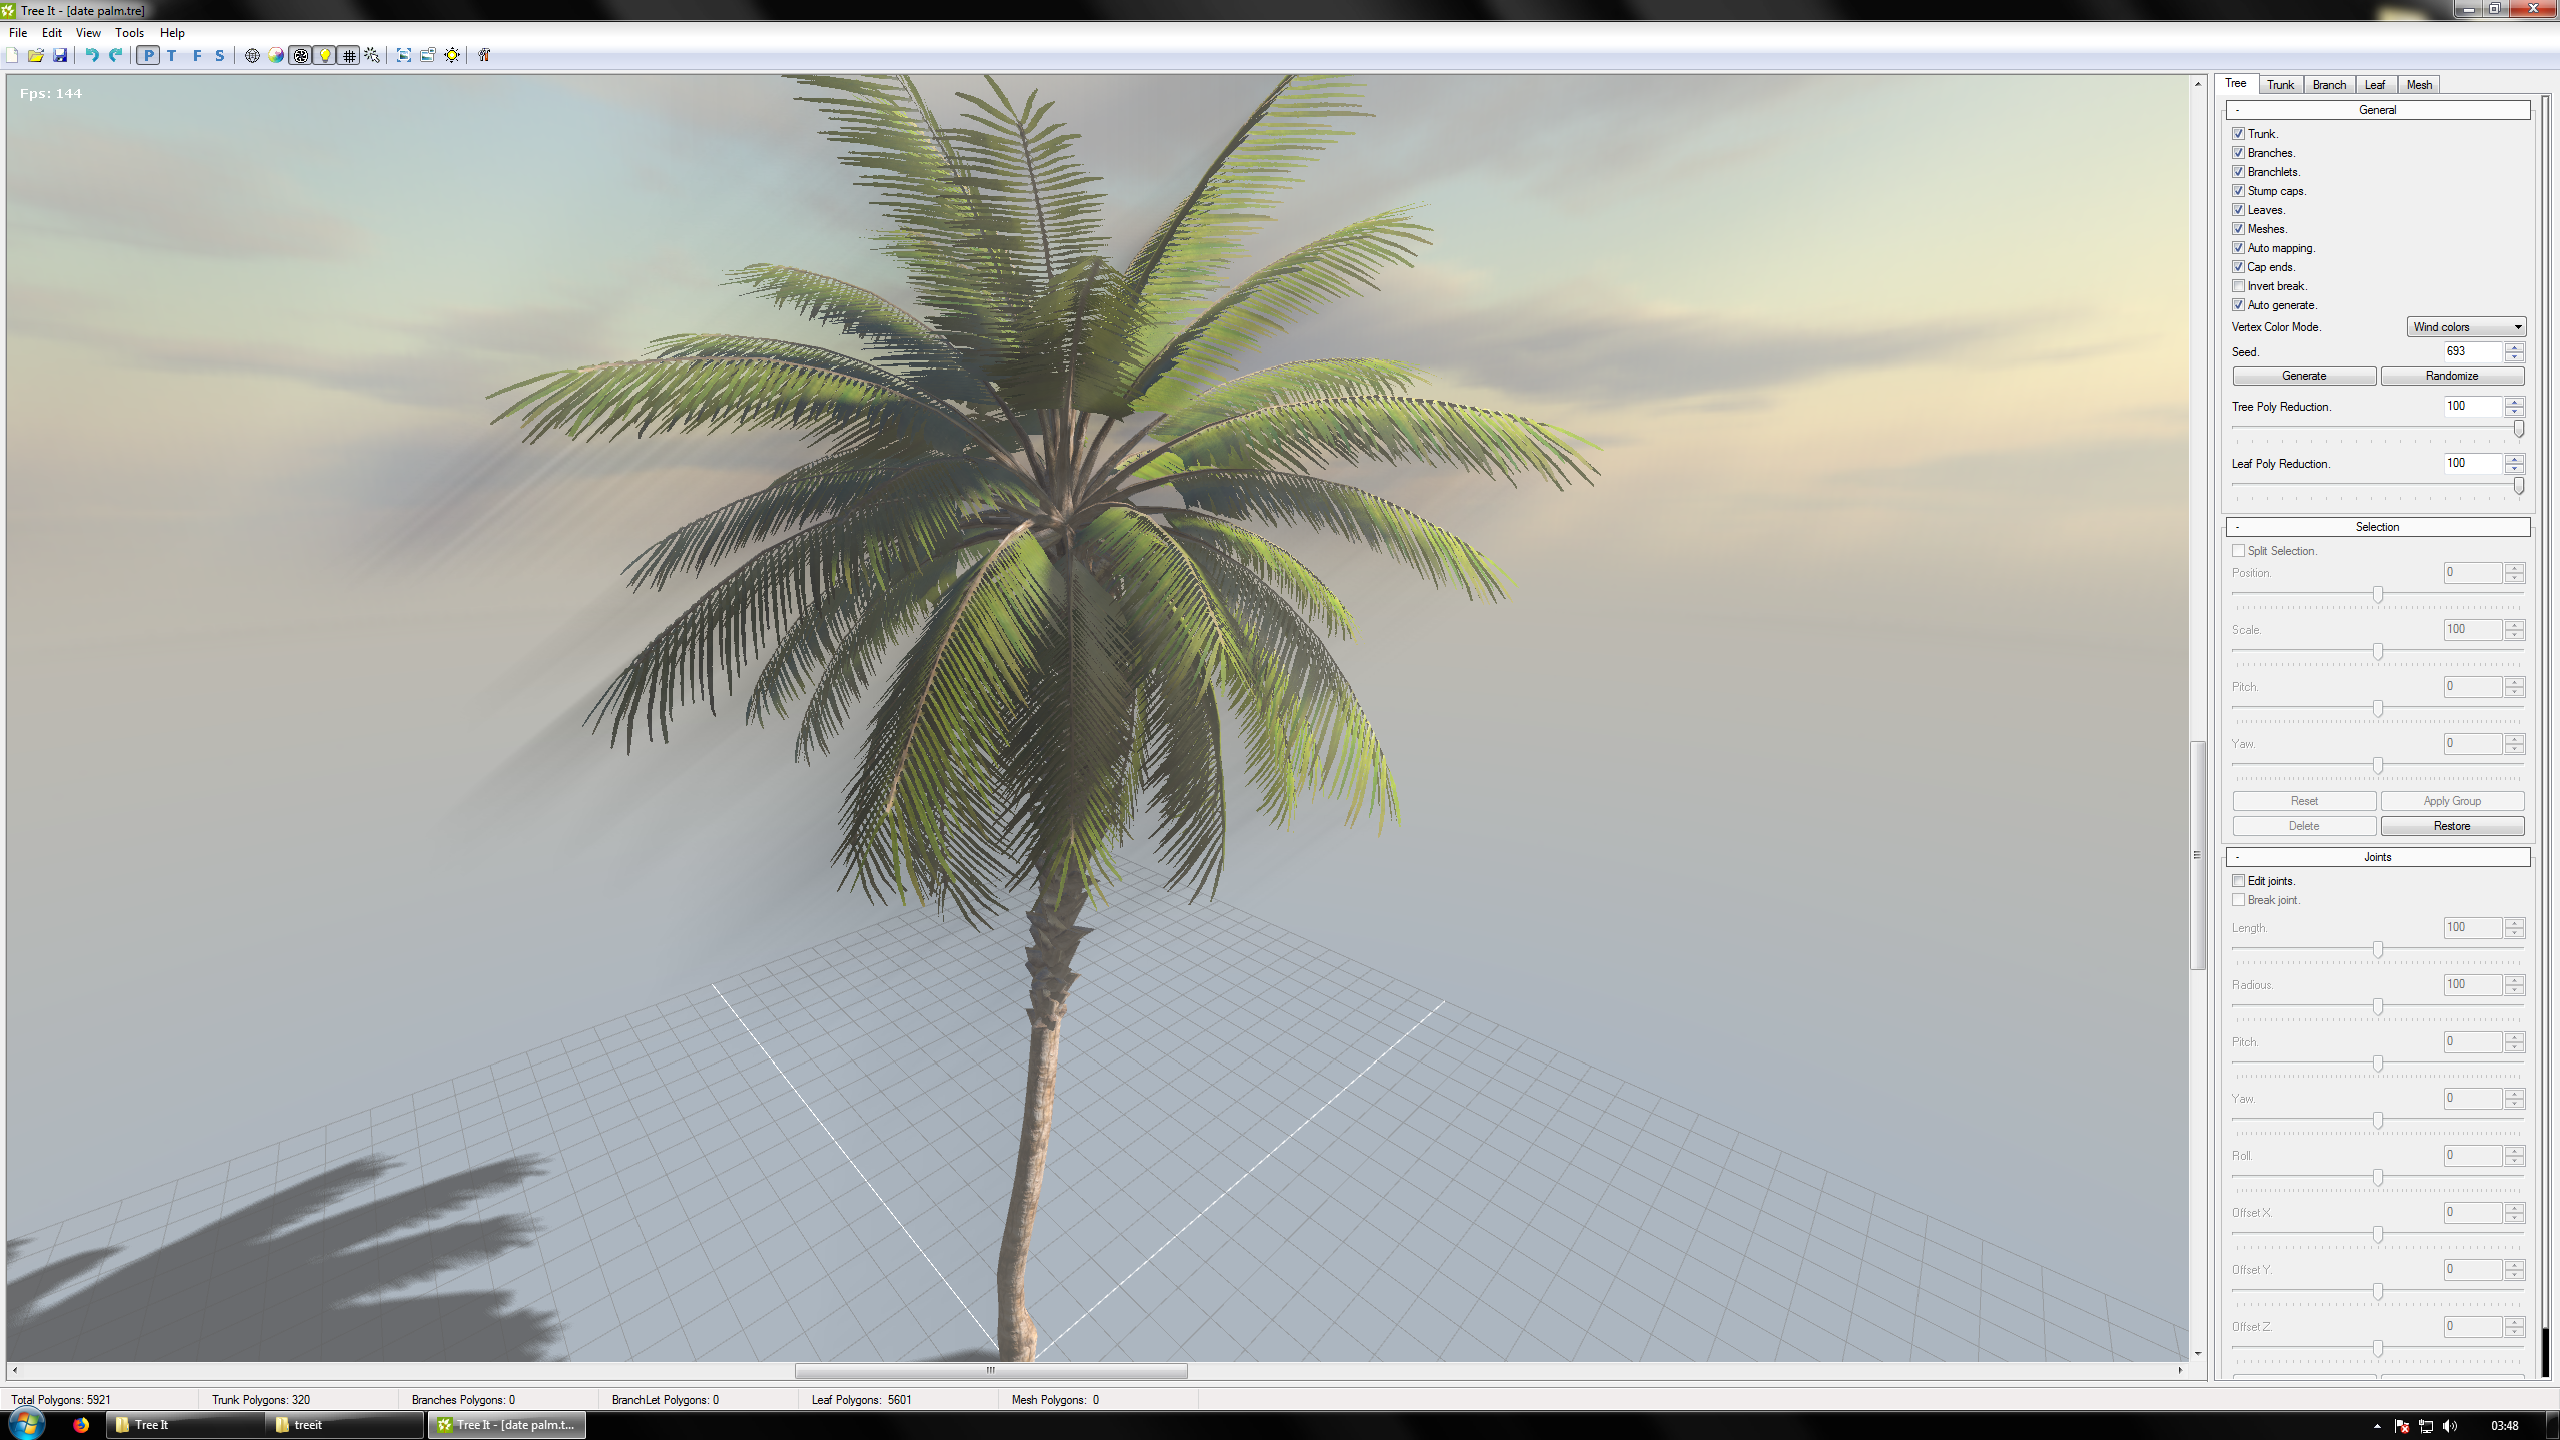
\includegraphics[width=0.8\textwidth]{treeit}
    \caption{Пример дерева, сгенерированного при помощи TreeIt.}
\end{figure}

\newpage
\section{TreeGen}
TreeGen - плагин для генерации деревьев в редакторе трёхмерных моделей Blender, распространяемый свободно по лицензии MIT.

TreeGen использует комбинацию из двух подходов: системы Линденмайера и параметрический подход.

\begin{figure}[h]
    \centering
    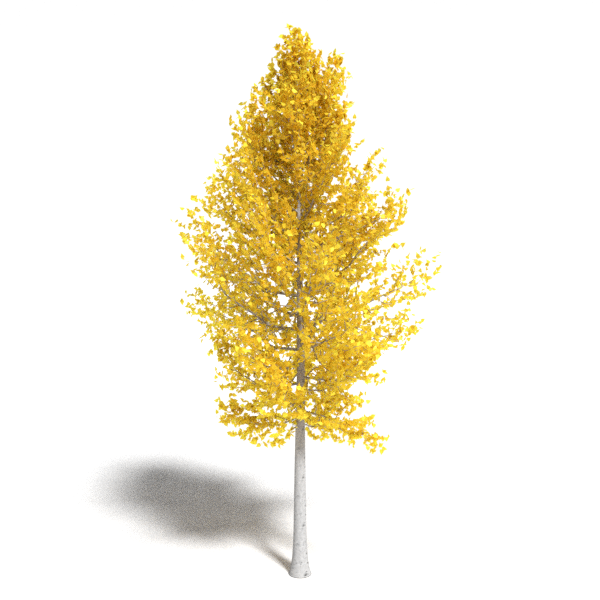
\includegraphics[width=0.8\textwidth]{treegen}
    \caption{Пример дерева, сгенерированного в плагине Treegen.}
\end{figure}

\section{Unity Tree Creator}

\newpage
